\documentclass[article,shortnames]{jss}
\usepackage[utf8]{inputenc}
\usepackage{natbib}
\usepackage{pdfpages}
\usepackage{xspace}
\usepackage{array}
\usepackage{tikz}
\usetikzlibrary{shapes.geometric, arrows}

\tikzstyle{io} = [trapezium, trapezium left angle=70, trapezium right angle=110, minimum width=3cm, minimum height=1cm, text centered, draw=black, fill=blue!30]
\tikzstyle{process} = [rectangle, minimum width=3cm, minimum height=1cm, text centered, draw=black, fill=orange!30]
\tikzstyle{decision} = [diamond, minimum width=3cm, minimum height=1cm, text centered, draw=black, fill=green!30]
\tikzstyle{arrow} = [thick,->,>=stealth]

\newcommand{\hl}[1]{\textcolor{magenta}{#1}}

\renewcommand\topfraction{.9}
\renewcommand\textfraction{.1}
\renewcommand{\floatpagefraction}{.6}
\renewcommand{\topfraction}{0.85}
\renewcommand{\bottomfraction}{0.85}
\renewcommand{\textfraction}{0.15}
\renewcommand{\floatpagefraction}{0.7}

%Virker ikke:
%\newcommand{\R}{\proglang{R}\xspace}

\newcommand{\R}[1]{\code{#1}}

\newcolumntype{L}[1]{>{\raggedright\let\newline\\\arraybackslash\hspace{0pt}}p{#1}}
\newcolumntype{C}[1]{>{\centering\let\newline\\\arraybackslash\hspace{0pt}}p{#1}}
\newcolumntype{R}[1]{>{\raggedleft\let\newline\\\arraybackslash\hspace{0pt}}p{#1}}


%%%%%%%%%%%%%%%%%%%%%%%%%%%%%%
%% declarations for jss.cls %%%%%%%%%%%%%%%%%%%%%%%%%%%%%%%%%%%%%%%%%%
%%%%%%%%%%%%%%%%%%%%%%%%%%%%%%

%% almost as usual
\author{Anne Helby Petersen\\Biostatistics\\Department of Public
  Health\\University of Copenhagen \And Claus Thorn Ekstr\o m\\Biostatistics\\Department of Public
  Health\\University of Copenhagen}
\title{\pkg{dataMaid}: your assistant for data documentation in \proglang{R}}

%% for pretty printing and a nice hypersummary also set:
\Plainauthor{Anne Helby Petersen, Claus Thorn Ekstr\o m} %% comma-separated
\Plaintitle{{dataMaid}: your assistant for data documentation in R} %% without formatting
\Shorttitle{\pkg{dataMaid}: your assistant for data documentation in R} %% a short title (if necessary)

%% an abstract and keywords
\Abstract{Data cleaning and -validation are important steps in any
  data analysis, as the validity of the conclusions from the analysis
  hinges on the quality of the input data. Mistakes in the data can
  arise for any number of reasons, including erroneous codings,
  malfunctioning measurement equipment, and inconsistent data generation
  manuals.  Ideally, a human investigator should go
  through each variable in the dataset and look for potential errors
  --- both in input values and codings --- but that process can be very
  time-consuming, expensive and error-prone in itself.

  We describe an \proglang{R} package, \pkg{dataMaid}, which
  implements an extensive and customizeable suite of quality
  assessment tools that can be applied to a dataset in order to
  identify potential problems in its variables. The results are 
  presented in an auto-generated, non-technical, stand-alone overview
  document intended to be perused by an investigator with an
  understanding of the variables in the data, but not necessarily
  knowledge of \proglang{R}. Thereby, \pkg{dataMaid} aids the dialogue
  between data analysts and field experts, while also providing easy
  documentation of reproducible data cleaning steps and data quality
  control. Moreover, the \pkg{dataMaid} solution changes the data
  cleaning process from the usual ad hoc approach to a systematic,
  well-documented endeavor.  \pkg{dataMaid} also provides a suite of
  more typical \proglang{R} tools for interactive data quality
  assessment and -cleaning, where the data inspections are executed directly 
  in the \proglang{R} console.

  % The \pkg{dataMaid} package is designed to be easily extended with
  % custom user-created checks that are relevant in particular
  % situations. \hl{Already said that above. Either expand on it or
  % delete this.}
}
\Keywords{data cleaning, quality control, \proglang{R}, data documentation}
\Plainkeywords{data cleaning, quality control, R, data documentation} %% without formatting
%% at least one keyword must be supplied

%% publication information
%% NOTE: Typically, this can be left commented and will be filled out by the technical editor
%% \Volume{50}
%% \Issue{9}
%% \Month{June}
%% \Year{2012}
%% \Submitdate{2012-06-04}
%% \Acceptdate{2012-06-04}

%% The address of (at least) one author should be given
%% in the following format:
\Address{
  Claus Thorn Ekstr\o m\\
  Biostatistics, Department of Public Health\\
  University of Copenhagen\\
  Denmark\\
  E-mail: \email{ekstrom@sund.ku.dk}\\
  URL: \url{http://staff.pubhealth.ku.dk/~ekstrom/}
}
%% It is also possible to add a telephone and fax number
%% before the e-mail in the following format:
%% Telephone: +43/512/507-7103
%% Fax: +43/512/507-2851

%% for those who use Sweave please include the following line (with % symbols):
%% need no \usepackage{Sweave.sty}

%% end of declarations %%%%%%%%%%%%%%%%%%%%%%%%%%%%%%%%%%%%%%%%%%%%%%%


\begin{document}


\section{Introduction}
Though data cleaning might be regarded as a somewhat tedious activity,
adequate data cleaning is crucial in any data analysis. With
ever-growing dataset sizes and complexities, statisticians and data
analysts find themselves spending a large portion of their time on
data cleaning and data wrangling. While a computer should generally not
make unsupervised decisions on what should be done to potential
errors in a dataset, it can still be an extremely useful tool in the
data cleaning process. Some errors can be tracked down and flagged by a
computer without further ado, while other types of errors need an analytic
context in order to be identified. Even in this latter case, well-designed
software can aid the process tremendously by providing the human
investigator with the information needed for identifying issues.

But even when tools are available for identifying problems in a dataset, the activity of data cleaning still suffers from a challenge that has recieved increasing attention in the scientitic communities in the later years: Data cleaning is not very straight forward to document and therefore, reproducibility suffers. \pkg{dataMaid}'s most central purpose is to facilitate a data cleaning workflow where documentation is thoroughly integrated rather than a secondary add-on. This is accomplished by centering the data cleaning process around auto-generated data overview reports that summarize the contents of the current version of a dataset and flags potential problems that could be candidates for the next bullet on the cleaning agenda. 

A number of \proglang{R} packages made for other pre-analysis tools are
already available, including \pkg{janitor} \citep{janitor}, \pkg{dplyr}
\citep{dplyr}, \pkg{tidyr}\citep{tidyr}, \pkg{data.table} \citep{data.table}, \pkg{DataCombine}
\citep{DataCombine} , \pkg{validate} \citep{validate}, \pkg{assertr} \citep{assertr}, and
\pkg{DataExplorer} \citep{DataExplorer}. These packages focus on
different stages of the pre-analysis work, most of which are not
really data cleaning.  \pkg{janitor} provides tools for data import
with a particular emphasis on the challenges of getting neat data
frames from Microsoft Excel data files. \pkg{dplyr}, \pkg{tidyr}, \pkg{data.table}
and \pkg{DataCombine} go a few steps further by providing a wide array
of extremely powerful tools for data wrangling, including a number of
particularly useful functions for merging and working with very large
datasets. When it comes to actual data cleaning, however, the options
are fewer.  \pkg{validate} (and the similar packages \pkg{editrules}
\citep{editrules} and \pkg{deducorrect} \citep{deducorrect} from the
same authors) does offer a few tools for identifying and
auto-correcting errors in a dataset, but, as the name suggests, the
focus is on internal validity rather than general data cleaning. In
practice, this means that quite elegant tools for, e.g., linear
restraints among the variables in a dataset can be applied, but
looking for potentially miscoded missing values is not really
feasible. The main difference between these two challenges is the
direction in which the data is inspected: While linear constraints
work observation-wise with no ambiguity, determining whether or not something
is a miscoded missing value often requires knowledge about the full
variable (e.g. range or data type), and thus it should be performed
variable-wise. \pkg{validate} does not allow for user-defined extensions
of the latter type, thereby limiting its data cleaning potential.
Automatic data correction functions are also provided by
\pkg{validate} which we consider to be quite a dangerous cocktail: all
power is given to the the computer with no human supervision, and
investigators are less likely to make an active, case-specific choice
regarding the handling of the potential errors.  Finally, no tools
have been made to easily document exactly which checks and preliminary
results were used in the data cleaning process. \hl{Something about \pkg{assertr} here.}

All in all, the large role of data cleaning in any data analysts
everyday endeavors is hardly matched in the amount of available
\proglang{R} software solutions. In particular, few packages attempt
to implement systematic, reproducible data cleaning. And while the
available tools attempt to alleviate the ubiquitous ad hoc approach to
data cleaning, they are primarily intended for the data savvy users
and less so for the general researcher with a knowledge about a
specific field and the context of the available data. The
\pkg{dataMaid} package \citep{dataMaid} presented here tries to address this by
providing a framework that both allows for extendable, systematic,
reproducible data cleaning, and summarizing findings for researchers
from other fields such that they can act as human experts when
tracking down potential errors.


One last package that should be mentioned in this context is
\pkg{DataExplorer} \citep{DataExplorer}. While this package does not
address data cleaning issues \emph{per se}, its general strategy is
quite similar to that of \pkg{dataMaid} and to the paradigms presented
below. This package provides a few simple, but practical, tools for
exploratory data analysis, including automated
documentation. Therefore, we find \pkg{DataExplorer} to be a good
candidate for a next-step package after data cleaning is finished.

But no matter how clever software tools we make, data cleaning remains
to be a time consuming endeavor, as it inherently requires human
interaction since every dataset is different and the variables in the
dataset can only be understood in the proper context of their
origin. This often requires a collaborative effort between an expert
in the field and a statistician or data scientist, which may be why
the process of proper data cleaning is not always undertaken. In many
situations, these errors are discovered in the process of the data
analysis (e.g., a categorical variable with numeric labels for each
category may be wrongly classified as a quantitative variable or a
variable where all values have erroneously been coded to the same
value), but in other cases a human with knowledge about the data
context area is needed to identify possible mistakes in the data
(e.g., if there are 4 categories for a variable that should only have
3).

The \pkg{dataMaid} approach to data cleaning, -quality assessment and -documentation is
governed by two fundamental paradigms. First of all, there is no need
for data cleaning to be an ad hoc procedure. Often, we have a very
clear idea of what flags are raisable in a given dataset before we
look at it, as we were the ones to produce it in the first place. This
means that data cleaning can easily be a well-documented,
well-specified procedure. In order to aid this paradigm, \pkg{dataMaid}
provides easy-to-use, automated tools for data quality assessment in
\proglang{R} \citep{R} on which data cleaning decisions can be made. This quality
assessment is presented in an auto-generated overview document,
readable by data analysts and field experts alike, thereby also
contributing to an inter-field dialogue about the data at
hand. Oftentimes, e.g., distinguishing between faulty codings of a
numeric value and unusual, but correct, values requires
problem-specific expertise that might not be held by the data
analyst. Hopefully, having easy access to data descriptions through
\pkg{dataMaid} will help this necessary knowledge sharing.

While \pkg{dataMaid}s primary raison d'être is auto-generating data
quality assessment overview documents, we still wish to emphasize that
it is \emph{not} a tool for unsupervised data cleaning. This qualifies
as the second paradigm of \pkg{dataMaid}: Data cleaning decisions
should always be made by humans. Therefore, \pkg{dataMaid} does not
supply any tools for ``fixing'' errors in the data. However, we do
provide interactive functions that can be used to identify potentially
erroneous entries in a dataset and that can make it easier to solve
data issues, one variable at a time.


This manuscript is structured as follows: First, in Section
\ref{sec:usingdataMaid}, we introduce the main representative of the first
paradigm, namely the \code{clean()} function, which generates data
overview documents. In the \pkg{dataMaid} package, we have
provided a number of default checks that cover the data
cleaning challenges, we find to be most common. Next, in Section
\ref{sec:interactiveCleanR}, we present the interactive mode of \pkg{dataMaid}, as motivated
by the second paradigm above. But, as any data analyst knows,
every dataset is different, and some datasets might include problems
that cannot be detected by our data checking functions. In Section
\ref{sec:extending}, we turn to the question of how \pkg{dataMaid} extensions
can be made, such that they are integrable with the \code{clean()}
function and with the other tools available in \pkg{dataMaid}.  At last,
in Section \ref{sec:specificExamples}, we discuss a number of examples of
specific data cleaning challenges and how \pkg{dataMaid} can be used to
solve them.

% \hl{Is there a Section 6?}

%\hl{Do they typically discuss notation in articles like this? I try (somewhat inconsistently) to refer to functions as \R{function()} while other \R{R} objects are referred to merely as \R{object}. This is also the style adopted by Wickham in his books.}


%% include your article here, just as usual
%% Note that you should use the \pkg{}, \proglang{} and \code{}
%% commands.


\section{Creating a data overview report}
\label{sec:usingdataMaid}

The \code{makeDataReport()} function is the primary workhorse of \pkg{dataMaid} and
this is the only function needed if a standard battery
of tests are used to generate data reports. The data report itself is an overview document, intended for reading
by humans, in either pdf or html format. Appendix \ref{sec:appendix1}
provides an example of a data report, produced by
calling \code{makeDataReport()} on the dataset \code{toyData} available in
\pkg{dataMaid}. The first two pages of this data report are
shown in Figure~\ref{fig:example1}. \code{toyData} is a very
small ($15$ observations of $6$ variables), artificial dataset which was created to
illustrate the main capabilities of \pkg{dataMaid}. The following
commands load the dataset and produce the report:

\begin{figure}[tb]
\begin{center}
\frame{\includegraphics[width=7.5cm,page=2]{dataMaid_toyData.pdf}}
\frame{\includegraphics[width=7.5cm,page=3]{dataMaid_toyData.pdf}}
%\includepdf[pages={2}, pagecommand={}]{dataMaid_testData.pdf}
\end{center}
\caption{Example output from running \code{makeDataReport()} on the \code{toyData}
  dataset. First a summary of the full dataset is given and then
  type-dependent information on each variable is given in a table and
  a graph. Larger versions of the pages can be seen in
  Appendix~\ref{sec:appendix1}.}
\label{fig:example1}
\end{figure}

\begin{Schunk}
\begin{Sinput}
R> library("dataMaid")
R> data("toyData")
R> toyData
\end{Sinput}
\begin{Soutput}
   var1 var2  var3       var4 var5       var6
1   red    1     a -0.6264538    1 Irrelevant
2   red    1     a  0.1836433    2 Irrelevant
3   red    1     a -0.8356286    3 Irrelevant
4   red    2     a  1.5952808    4 Irrelevant
5   red    2     a  0.3295078    5 Irrelevant
6   red    6     b -0.8204684    6 Irrelevant
7   red    6     b  0.4874291    7 Irrelevant
8   red    6     b  0.7383247    8 Irrelevant
9   red  999     c  0.5757814    9 Irrelevant
10  red   NA     c -0.3053884   10 Irrelevant
11 blue    4     c  1.5117812   11 Irrelevant
12 blue   82     .  0.3898432   12 Irrelevant
13 blue   NA       -0.6212406   13 Irrelevant
14 <NA>  NaN other -2.2146999   14 Irrelevant
15 <NA>    5 OTHER  1.1249309   15 Irrelevant
\end{Soutput}
\end{Schunk}
\begin{Schunk}
\begin{Sinput}
R> makeDataReport(toyData)
\end{Sinput}
\end{Schunk}

By default, an \proglang{R} markdown file and a rendered pdf overview
document is produced, saved to the working directory and
opened for immediate inspection. Turning to Figure~\ref{fig:example1},
we see that such a data report consists of three
parts. First, an overview of what was done is presented under the
title \textit{Data report overview}. Secondly, an index listing each variable along with an indication of whether it was found to be problematic or not is provided. Thirdly, each variable in the
dataset is presented in turn using (up to) three tools in the
\textit{Variable list}: A table summarizing key features of the
variable, a figure visualizing its distribution and a
list of flagged issues, if any. For instance, in the \code{numeric}-type variable
\code{var2} from \code{toyData}, \code{makeDataReport()} has identified two values that
are suspected to be miscoded missing values (\code{999} and \code{NaN}),
while two values were also flagged as potential outliers that should
be investigated more carefully.

Though the \code{makeDataReport()} function is very easy to use, it should not be
mistaken to be inflexible: By using the optional arguments of the function, 
both the contents and the look of the data report can be molded 
according to the user's needs. The most commonly used arguments are summarized in
Table~\ref{table.cleanFormals} and they are grouped according to the
part of the data assesment and report generation they influence. In order to understand
this distinction, a glimpse of the inner structure of \code{makeDataReport()} is
shown in Figure~\ref{figure:cleanStructure}. Below, we present a few
examples on how to use the arguments from Table \ref{table.cleanFormals}
 to influence the output of a \code{makeDataReport()} call.

\begin{table}
\small
\begin{tabular}{p{0.25\linewidth}p{0.45\linewidth}p{0.2\linewidth}}
\hline
Argument & Description & Default value \\
\hline

\smallskip Control input variables and summary\\
\quad \code{useVar} & What variables should be used? & \code{NULL} (corresponding to all variables) \\
\quad \code{ordering} & Ordering of the variables in the data summary (as is or alphabetical) & \code{"asIs"} \\
\quad \code{onlyProblematic} & Should only variables flagged as problematic be included in the \textit{Variable list}? & \code{FALSE} \\
\quad \code{listChecks} & Should an overview of what checks were performed be listed in the \textit{Data report overview}? &  \code{TRUE} \\
\quad \code{preChecks} & What check functions should be called to determine whether a variable is suitable for summarization, visualization and checking? & \code{c("isKey", "isEmpty")} \\

\smallskip Control summarize, visualize, and check steps \\
\quad \code{mode} & What steps should be performed for each variable (out
                 of the three possibilities \textit{summarize},
                 \textit{visualize}, \textit{check})? &
                                                        \code{c("summarize", "visualize", "check")} (corresponding to all three steps) \\
\quad \code{smartNum} & Should numerical values with only a few unique
                     levels be flagged and treated as a factor variable? & \code{TRUE} \\
\quad \code{maxProbVals} & Maximum number of problematic values to print, if any are found in data checks & \code{Inf} \\
\quad \code{maxDecimals} & Maximum number of decimals to print for numeric values in the variable list & \code{2} \\
\quad \code{twoCol} & Should the summary table and visualizations be placed side-by-side (in two columns)? & \code{TRUE} \\

\smallskip Control output and post-processing \\
\quad \code{output} & Type of output file to be produced (html, or pdf) & \code{"pdf"} \\
\quad \code{render} & Should the output file be rendered from markdown? & \code{TRUE} \\
\quad \code{openResult} & If a  pdf/html file is rendered, should it
                       automatically open afterwards, and if not,
                       should the \code{rmarkdown} file be opened? & \code{TRUE} \\
\quad \code{replace} & Overwrite an existing file with the same name? & \code{FALSE} \\

\hline
\end{tabular}
\caption{A selection of commonly used arguments to \code{makeDataReport()} separated into the parts they control.}
\label{table.cleanFormals}
\end{table}

\begin{figure}[tb]
% Define block styles
\tikzstyle{decision} = [diamond, draw, fill=blue!20,
    text width=5.5em, text badly centered, node distance=3cm, inner
    sep=0pt]
\tikzstyle{block} = [rectangle, draw, fill=blue!20,
    text width=6em, text centered, rounded corners, minimum
    height=4em]
\tikzstyle{line} = [draw, -latex']
\tikzstyle{cloud} = [draw, ellipse,fill=red!20, node distance=3cm,
    text width=5em,
    minimum height=2em]

\begin{center}
\begin{tikzpicture}[node distance = 2cm, auto,thick,scale=0.75, every node/.style={transform shape}]
    % Place nodes
    \node [block] (init) {Get next variable and run pre-checks};
    \node [cloud, above of=init] (input) {Input \code{data.frame} or \code{tibble}};
%    \node [cloud, right of=init] (system) {system};
    \node [decision, right of=init, node distance=4cm] (precheck) {Is variable suitable for inclusion};
    \node [block, right of=precheck, node distance=4cm] (summarize)
    {Run \code{summarize()} to produce summary table};
    \node [block, below of=summarize, node distance=3cm] (visualize)
    {Run \code{visualize()} to plot variable};
    \node [block, below of=visualize, node distance=2.5cm] (check)
    {Call \code{check()} to run error checks};
    \node [decision, below of=check, node distance=2.7cm] (done) {More
      variables?};
    \node [block, right of=done, node distance=3.5cm] (stop) {Write
      \proglang{R} markdown file};
    \node [cloud, below of=stop, node distance=3.5cm] (render) {Render
      markdown and possiby open};
    % Draw edges
    \path [line] (summarize) -- (visualize);
    \path [line] (visualize) -- (check);
    \path [line] (check) -- (done);
    \path [line] (done.south) -- +(0,-10pt) -| node [near start] {yes} (init);
%    \path [line] (identify) -- (evaluate);
%    \path [line] (evaluate) -- (decide);
%    \path [line] (init) -| node [near start] {yes} (precheck);
    \path [line] (init) -- (precheck);
    \path [line] (precheck) -- node [near start] {yes} (summarize);
    \path [line] (precheck) |- node [near start] {no} (done);
    \path [line] (done) -- node [near start] {no} (stop);
%    \path [line] (update) |- (identify);
%    \path [line] (decide) -- node {no}(stop);
    \path [line,dashed] (input) -- (init);
    \path [line] (stop) -- (render);
%    \path [line,dashed] (system) -- (init);
%    \path [line,dashed] (system) |- (evaluate);
\end{tikzpicture}
\end{center}

\caption{Schematic illustration of the stages undertaken when running
  \code{makeDataReport()}. Each variable is checked for eligibility before
  running \code{summarize()}, \code{visualize()}, and \code{check()}, and the
  resulting \proglang{R} markdown file may be rendered and opened.}
\label{figure:cleanStructure}
\end{figure}




% \subsection{Controlling [something]}
% \label{subsection:controlSomething}

\subsection{Polishing off the arguments}
We begin with an example that is intended as an illustration of how
\code{makeDataReport()} might be used in the very first stages of data
cleaning, when the we are uncertain about the complexities of the
errors and how much time should be allocated to data cleaning. At
this stage, what is really needed, is a very rough idea of the
severity of errors in the dataset. In this scenario, we might wish to
obtain a summary document in html format that only contains the
variables with potential problems, and with a limit of, say, maximum
10 printed potential errors for each variable. Also, we can add the
argument \code{replace=TRUE} in order to force \code{makeDataReport()} to
overwrite any existing files produced by \code{makeDataReport()}.  Using the
\code{toyData} dataset as a guinea pig, we type:

\begin{Schunk}
\begin{Sinput}
R> makeDataReport(toyData, output = "html", onlyProblematic = TRUE, maxProbVals = 10,
+    replace = TRUE)
\end{Sinput}
\end{Schunk}

The final rendering of the generated markdown file is controlled by
the \code{render} and \code{openResult} arguments, which both default to
\code{TRUE}. \code{render} determines if the \proglang{R} markdown file
produced should be rendered using the \pkg{rmarkdown} \citep{rmarkdown} package and
\code{openResult} decides whether the output html or pdf file should be
opened. The following command produces an \proglang{R} markdown file
containing the information needed for generating a data report, but without
rendering nor opening the markdown file:

\begin{Schunk}
\begin{Sinput}
R> makeDataReport(toyData, output="html", render=FALSE, openResult=FALSE)
\end{Sinput}
\end{Schunk}


\begin{table}
\centering
\begin{tabular}{p{0.35\linewidth} p{0.3\linewidth} p{0.01\linewidth} p{0.01\linewidth} p{0.01\linewidth} p{0.01\linewidth} p{0.01\linewidth}
 p{0.01\linewidth} p{0.01\linewidth}}
  \hline
& Description &  \multicolumn{7}{c}{Variable classes} \\ \smallskip
 & &  C & F & I & L & B & N & D\\
  \hline \smallskip
  \textbf{\code{summaryFunction}s}  \smallskip \\
  \quad \code{centralValue} & Compute median or mode &  $\times$ & $\times$ & $\times$ & $\times$ & $\times$ & $\times$ & $\times$ \\
  \quad \code{countMissing} & Compute proportion of missing observations &  $\times$ & $\times$ & $\times$ & $\times$ & $\times$ & $\times$ & $\times$  \\
  \quad \code{minMax} & Find minimum and maximum values &   &  & $\times$ & &  & $\times$ & $\times$  \\
  \quad \code{quartiles} & Compute 1st and 3rd quartiles &    &  & $\times$ & &  & $\times$ & $\times$ \\
  \quad \code{uniqueValue} & Count number of unique values &   $\times$ & $\times$ & $\times$ & $\times$ & $\times$ & $\times$ & $\times$  \\
  \quad \code{variableType} & Data class of variable & $\times$ & $\times$ & $\times$ & $\times$ & $\times$ & $\times$ & $\times$  \\
  \smallskip \\
 \textbf{\code{visualFunction}s} \smallskip \\
  \quad \code{basicVisual} & Histograms and barplots using base \proglang{R} graphics &  $\times$ & $\times$ & $\times$ & $\times$ & $\times$ & $\times$ & $\times$ \\
  \quad \code{standardVisual} & Histograms and barplots using \pkg{ggplot2} &  $\times$ & $\times$ & $\times$ & $\times$ & $\times$ & $\times$ & $\times$ \\
  \smallskip \\
 \textbf{\code{checkFunction}s} \smallskip \\
 \quad \code{identifyCaseIssues} & Identify case issues &  $\times$ & $\times$ & & & & &  \\
 \quad \code{identifyLoners} & Identify levels with $<$ 6 obs. & $\times$ & $\times$ & & & & &  \\
 \quad \code{identifyMissing} & Identify miscoded missing values &  $\times$ & $\times$ & $\times$ & $\times$ & $\times$ & $\times$ &  \\
 \quad \code{identifyNums} & Identify misclassified numeric or integer variables & $\times$ & $\times$ & & & & &  \\
 \quad \code{identifyOutliers} & Identify outliers &  & & $\times$ & & $\times$ & $\times$ \\
 \quad \code{identifyOutliersTBStyle} & Identify outliers (Turkish Boxplot style) &  & & $\times$ & & $\times$ & $\times$ \\
 \quad \code{identifyWhitespace} & Identify prefixed and suffixed whitespace &  $\times$ & $\times$ & & $\times$ & & &  \\
 \quad \code{isCPR} & Identify Danish CPR numbers & $\times$ & $\times$ & $\times$ & $\times$ & $\times$ & $\times$ &$\times$   \\
 \quad \code{isEmpty} & Check if the variable contains only a single value & $\times$ & $\times$ & $\times$ & $\times$ & $\times$ & $\times$ & $\times$  \\
 \quad \code{isKey} & Check if the variable is a key & $\times$ & $\times$ & $\times$ & $\times$ & $\times$ & $\times$ & $\times$\smallskip   \\
 \hline
\end{tabular}
\caption{List of all summary functions (used in the summary table for
  each variable in the output), visual functions (used for  visualization of each variable), and
  check functions (used for data checks for each variable) currently implemented in \pkg{dataMaid}. The variable
  classes C, F, I, L, B, N, and D, refer to \code{character}, \code{factor},
  \code{integer}, \code{labelled}, \code{logical} (boolean), \code{numeric}, and \code{Date}, respectively.}
\label{table.SVCfunctions}
\end{table}


We will now move on to discuss how not only the structure of the
data assesment steps is manipulated, but also its very contents. This is
done through the summarize/visualize/check (SVC) steps, as illustrated
in Figure \ref{figure:cleanStructure}.  \pkg{dataMaid} uses three
different types of functions for performing these steps, namely
\code{summaryFunction}s, \code{visualFunction}s and
\code{checkFunction}s.  By default, \code{clean()} runs selected summary,
visualization and check functions on each variable in the dataset, and
the exact choice of these functions depends on the classes of the
variables. For instance, though detection of outlier values might be
interesting for numerical variables, it holds little meaning for
factor variables, and therefore, numerical and factor variables need
different checks. Table~\ref{table.SVCfunctions} lists all available
summarize/visualize/check functions, but we can also use the
\code{allSummaryFunctions()}, \code{allVisualFunctions()}, and
\code{allCheckFunctions()} functions in \pkg{dataMaid} to print overview
lists in \proglang{R}. For example, the implemented
\code{summaryFunction}s are:

%\subsection{Something about what check, visual and summary functions are available}

\begin{Schunk}
\begin{Sinput}
R> allSummaryFunctions()
\end{Sinput}
\begin{Soutput}
----------------------------------------------------------------------------
name           description                     classes                      
-------------- ------------------------------- -----------------------------
centralValue   Compute median or mode          character, Date, factor,     
                                               integer, labelled, logical,  
                                               numeric                      

countMissing   Compute proportion of missing        character, Date, factor,     
               observations                    integer, labelled, logical,  
                                               numeric                      

minMax         Find minimum and maximum        integer, numeric, Date       
               values                                                       

quartiles      Compute 1st and 3rd quartiles   Date, integer, numeric       

uniqueValues   Count number of unique values   character, Date, factor,     
                                               integer, labelled, logical,  
                                               numeric                      

variableType   Data class of variable          character, Date, factor,     
                                               integer, labelled, logical,  
                                               numeric                      
----------------------------------------------------------------------------
\end{Soutput}
\end{Schunk}

Thus we can see, for example, that for \code{numeric}, \code{integer},
and \code{Date} variables, \pkg{dataMaid} provides functions for
adding summary information about the minimum and maximum values, while
all seven variable classes dealt with in \pkg{dataMaid} have functions
for central tendency summaries (i.e., mode or median).

We can control what summaries and checks are applied for each variable type
through the \code{summaries}, \code{visuals} and \code{checks} arguments. Each of these arguments should be a list with one entry for each variable type and a number of function names for each such entry. The easiest way to specify the arguments is by use of the built-in helper functions \code{setSummaries()}, \code{setVisuals()} and \code{setChecks()}. 

For instance, we can inspect the default settings for summaries by calling

\begin{Schunk}
\begin{Sinput}
R> setSummaries()
\end{Sinput}
\begin{Soutput}
$character
[1] "identifyMissing"  "identifyWhitespace"  "identifyLoners"    
[4]  "identifyCaseIssues"  "identifyNums"      

$factor
[1] "identifyMissing"  "identifyWhitespace"  "identifyLoners"     
[4] "identifyCaseIssues"  "identifyNums"      

$labelled
[1] "identifyMissing"  "identifyWhitespace"  "identifyLoners"     
[4] "identifyCaseIssues"  "identifyNums"      

$numeric
[1] "identifyMissing"  "identifyOutliers"

$integer
[1] "identifyMissing"  "identifyOutliers"

$logical
NULL

$Date
[1] "identifyOutliers"
\end{Soutput}
\end{Schunk} %$

This helper function really just calls several other helper functions, namely the \\ 
\code{defaultXXXSummaries()} functions, where \code{XXX} refers to a variale class. For instance, we can see the default character checks by calling \code{defaultCharacterSummaries()}:

\begin{Schunk}
\begin{Sinput}
R> defaultCaracterSummaries()
\end{Sinput}
\begin{Soutput}
[1] "variableType" "countMissing" "uniqueValues" "centralValue"
\end{Soutput}
\end{Schunk}

We can change the choice of summaries (and similarly the checks and visual functions) by setting the
corresponding arguments when calling \code{makeDataReport()}. For example, to get
only the variable type and the central tendency listed in the summary
table for numeric and integer variables, we write

\begin{Schunk}
\begin{Sinput}
R> makeDataReport(toyData, 
 	summaries = setSummaries(numeric = c("variableType","centralValue),
		integer = c("variableType", "centralValue"))
\end{Sinput}
\end{Schunk}

In the case where we specify the same set of summary
functions for each variable type, we can use a simpler argument for \code{setSummaries} which overrides the summary functions for all
variable types:

\begin{Schunk}
\begin{Sinput}
R> makeDataReport(toyData, 
	summaries = setSummaries(all = c("variableType", "centralValue"))
\end{Sinput}
\end{Schunk}

Similarly, the checks applied are set with the \code{checks} argument and the \code{setChecks} function. The default checks being applied to a factor are

\begin{Schunk}
\begin{Sinput}
R> defaultFactorChecks()
\end{Sinput}
\begin{Soutput}
[1] "identifyMissing"    "identifyWhitespace" "identifyLoners"    
[4] "identifyCaseIssues" "identifyNums"      
\end{Soutput}
\end{Schunk}

Now, if we only wanted to apply the function to identify whitespace
for factor variables, then we would need provide this information for \code{setChecks()}:

\begin{Schunk}
\begin{Sinput}
R> makeDataReport(toyData, checks = setChecks(factor = "identifyWhitespace"))
\end{Sinput}
\end{Schunk}

or we could remove checks for factors altogether by setting the
corresponding argument to \code{NULL}, in which case factor variables will
not be checked for any potential errors:

\begin{Schunk}
\begin{Sinput}
R> makeDataReport(toyData, checks = setChecks(factor = NULL))
\end{Sinput}
\end{Schunk}

As with \code{summaryFunction}s, a complete list of available
\code{checkFunction}s is obtained by calling
\code{allCheckFunctions()}. Note however, that \code{checkFunction}s have a
usage beyond the \code{checks} arguments, namely in the
pre-check stage. In this stage, it is determined whether or
not each variable is suitable for the summarize/visualize/check (SVC)
steps. The functions used in the pre-check stage should be
\code{checkFunction}s that are applicable to all variable classes. The
default pre-checks, the functions \code{isKey()} and \code{isSingular()}, check
whether a variable has unique values for all observations or only a
single value for all observations, respectively. If one of these
statements are true, the variable will not be subjected to the SVC
steps.  We can allow empty variables to move on to the SVC step by
only checking for keys in the pre-check step:

\begin{Schunk}
\begin{Sinput}
R> makeDataReport(toyData, preChecks = "isKey")
\end{Sinput}
\end{Schunk}

Note that the data visualizations in the cleaning summary are also
controllable, though only a single function can be provided for each variable type. If, for instance, we wish to change the visualizations
from the default \pkg{ggplot2} \citep{ggplot2} style histograms and barplots to base
\proglang{R} histograms and barplots, we type

\begin{Schunk}
\begin{Sinput}
R> makeDataReport(toyData, visuals = setVisuals(all = "basicVisual"))
\end{Sinput}
\end{Schunk}


As indicated in Figure~\ref{figure:cleanStructure}, there are two stages
where \code{makeDataReport()} applies functions to each of the variables:
\begin{enumerate}
\item In the pre-check stage.
\item As part of the summarize/visualize/check (SVC) steps.
\end{enumerate}
Each of these stages are controllable using appropriate function
arguments in \code{makeDataReport()}, and above we have shown examples of how
to tweak them to modify the data cleaning outputs. However, if the
dataset at hand requires new, additional checks, then more control is
needed \hl{ and we have provided a detailed vignette that explains how to modify and
expand the possibilities by producing new summary, visual, and check
functions in [REFERENCE]}.


\section[Using dataMaid interactively]{\hl{Using \pkg{dataMaid} interactively}}
\label{sec:interactiveCleanR}

While overview documents are great for presenting and documenting the
data cleaning checks, it may be useful to be able to work more
interactively through the data cleaning process. Aside from
the \code{clean()} function presented above, \pkg{dataMaid} also
provides more standard \proglang{R} interactive tools, such as
functions that print results to the console or return the information
as an object for later use. This section describes how to use the
functions \code{check()}, \code{summarize()} and \code{visualize()} to
work interactively with \pkg{dataMaid}.

\subsection{Data cleaning by hand: An example}
Assume that we wish to look further into a certain variable from
\code{toyData}, namely \code{var2}. The data cleaning summary found some
issues in this variable, and we would like to recall what these issues
were. This can be done using the \code{check()} command

\begin{Schunk}
\begin{Sinput}
R> check(toyData$var2)
\end{Sinput}
\begin{Soutput}
$identifyMissing
The following suspected missing value codes enter as regular values: 999, NaN.
$identifyOutliers
Note that the following possible outlier values were detected: 82, 999.
\end{Soutput}
\end{Schunk}%$

Note that the arguments specifying which checks to perform, as
described in the previous section, are in fact passed to \code{check()},
and thus they can also be used here. For instance, if we only want to
check for potentially miscoded missing values, we can use the relevant
\code{XXXChecks} argument (e.g., \code{numericChecks}, \code{factorChecks},
etc., as described in Section~\ref{sec:usingdataMaid}) to provide a
vector of the check functions that should be applied. Recall that
Table~\ref{table.SVCfunctions} or an \code{allCheckFunctions()} call provide
overviews of the available check functions.
Moving forward, we limit the numeric checks to only identify miscoded
missing values:

\begin{Schunk}
\begin{Sinput}
R> check(toyData$var2, numericChecks = "identifyMissing")
\end{Sinput}
\begin{Soutput}
$identifyMissing
The following suspected missing value codes enter as regular values: 999, NaN.
\end{Soutput}
\end{Schunk}

An equivalent way to call only a single, specific \code{checkFunction},
such as \code{identifyMissing}, is by using it directly on the variable,
e.g.,

\begin{Schunk}
\begin{Sinput}
R> identifyMissing(toyData$var2)
\end{Sinput}
\begin{Soutput}
The following suspected missing value codes enter as regular values: 999, NaN.
\end{Soutput}
\end{Schunk}

The result of a \code{checkFunction} is an object of class
\code{checkResult}. By using the structure function, \code{str()}, we can
look further into its components:

\begin{Schunk}
\begin{Sinput}
R> missVar2 <- identifyMissing(toyData$var2)
R> str(missVar2)
\end{Sinput}
\begin{Soutput}
List of 3
 $ problem      : logi TRUE
 $ message      : chr "The following suspected missing value codes
    enter as regular values: \\\"999\\\", \\\"NaN\\\"."
 $ problemValues: num [1:2] 999 NaN
 - attr(*, "class")= chr "checkResult"
\end{Soutput}
\end{Schunk}

The most important thing to note here is that while the printed
message is made for easy reading, the actual values of the variable
causing the issue are still obtainable in the element
\code{problemValues}. If we decide that the values \code{999}
and \code{NaN} in \code{var2} are in fact miscoded missing values, we can
easily replace them with \code{NA}s:

\begin{Schunk}
\begin{Sinput}
R> toyData$var2[toyData$var2 %in% missVar2$problemValues] <- NA
R> identifyMissing(toyData$var2)
\end{Sinput}
\begin{Soutput}
No problems found.
\end{Soutput}
\end{Schunk}

Similarly, the \code{visualize()} and \code{summarize()} functions can be
used to run the corresponding visualizations and summaries for each
variable. See Figure~\ref{fig:example2} for the visualization output.

\begin{Schunk}
\begin{Sinput}
R> visualize(toyData$var2)
R> summarize(toyData$var2)
\end{Sinput}
\begin{Soutput}
     Feature                   Result       
[1,] "Variable type"           "numeric"    
[2,] "Number of missing obs."  "4 (26.67 %)"
[3,] "Number of unique values" "6"          
[4,] "Median"                  "4"          
[5,] "1st and 3rd quartiles"   "1.5; 6"     
[6,] "Min. and max."           "1; 82"      
\end{Soutput}
\end{Schunk}

\begin{figure}[tb]
\begin{center}
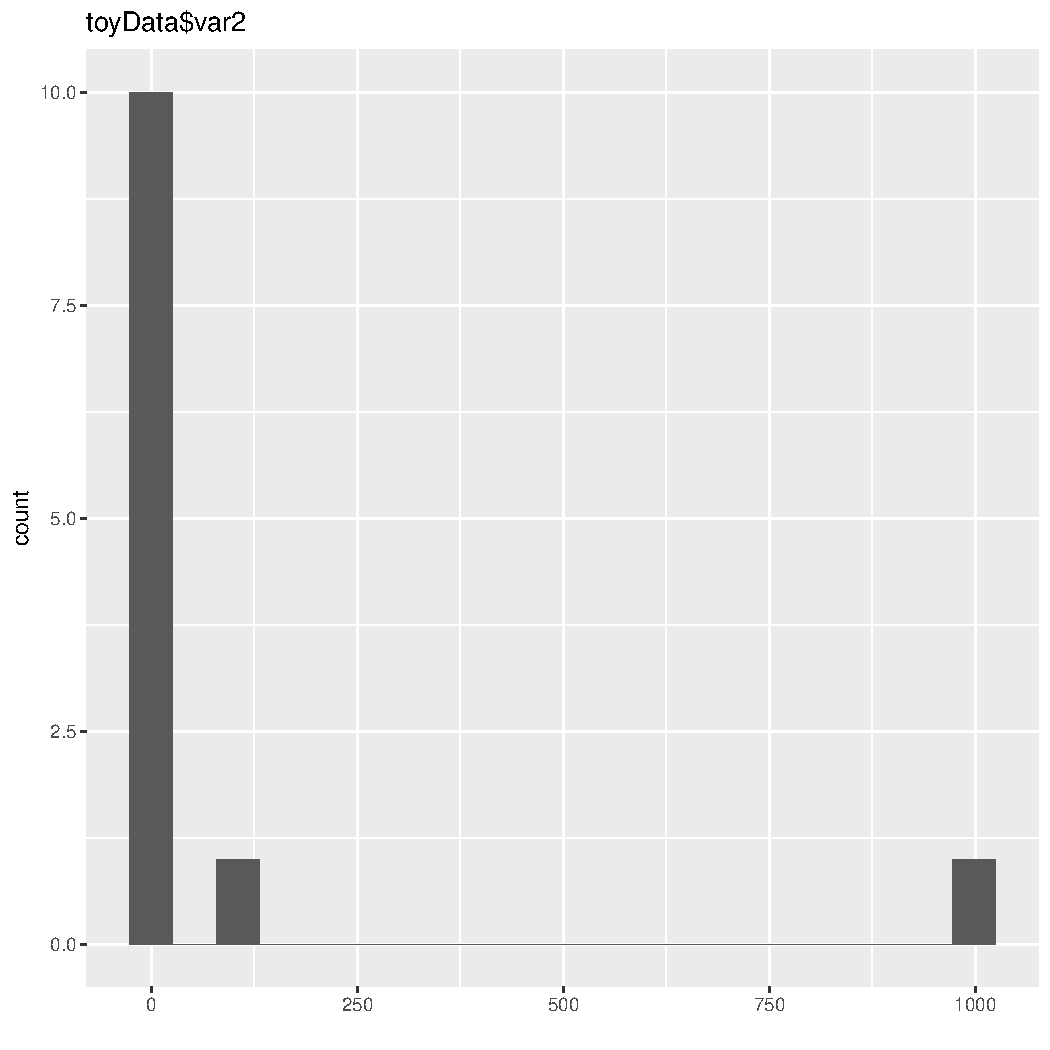
\includegraphics[width=7.5cm]{toyData-var2.pdf}
\end{center}
\caption{Output from running \code{visualize()} on the variable \code{var2} from the
\code{toyData} dataset.}
\label{fig:example2}
\end{figure}


As we saw with the \code{check()} function, the summary can be modified
by providing the relevant \code{XXXSummaries} arguments. Setting the
\code{numericSummaries} argument, we can control the summary output by
providing a vector of function names to run for a particular summary. To
only get the median, minimum and the maximum we set
\code{numericSummaries = c("centralValue", "minMax")}:

\begin{Schunk}
\begin{Sinput}
R> summarize(toyData$var2, numericSummaries = c("centralValue", "minMax"))
\end{Sinput}
\begin{Soutput}
     Feature         Result 
[1,] "Median"        "4"    
[2,] "Min. and max." "1; 82"
\end{Soutput}
\end{Schunk}

Note that the \code{summarize()}, \code{check()} and \code{visualize()} functions are also available interactively for full datasets by calling e.g., \code{summarize(toyData)}. However, this produces an extensive amount of output in the console, and therefore, we generally do not recommend it, unless working with very small datasets or subsets of datasets.

\section{A worked example: Dirty presidents} 
\label{sec:bigExample}
\hl{Er titlen her for popsmart og flabet? Det er måske også et generelt tema i teksten. Ret gerne kritisk.}

\begin{figure}[tb]
\begin{center}
\frame{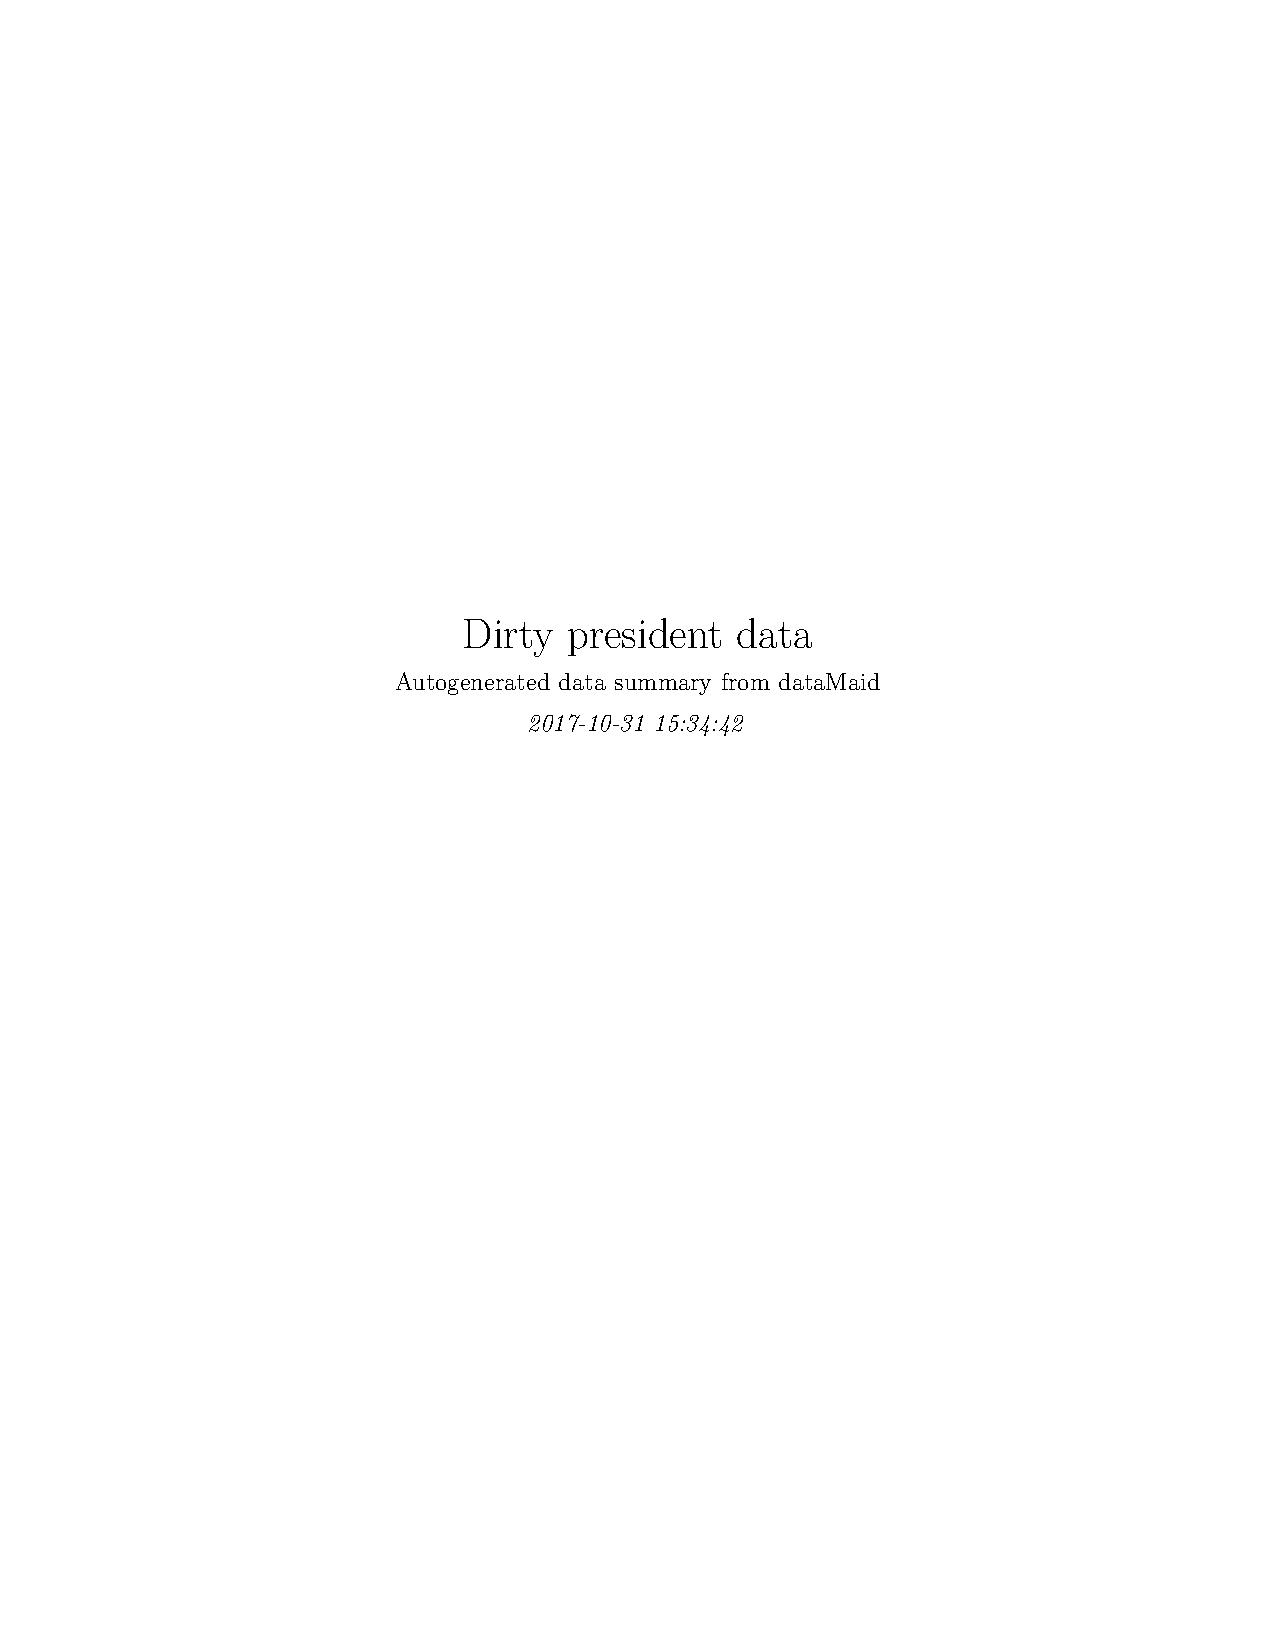
\includegraphics[width=7.5cm,page=1]{dataMaid_presidentData.pdf}}
\frame{\includegraphics[width=7.5cm,page=2]{dataMaid_presidentData.pdf}}\\
\frame{\includegraphics[width=7.5cm,page=3]{dataMaid_presidentData.pdf}}
\frame{\includegraphics[width=7.5cm,page=4]{dataMaid_presidentData.pdf}}
\end{center}
\caption{The first 4 pages of the data overview report for the \code{presidentData} dataset. Note that the report title has been customized (front page), \code{identifyLoners} has been removed from the checks performed on character variables (page 1) and that variables of class \code{Name} have been set to be treated like \code{character} variables (page 1). We see that there are two \code{Name} variables in the overview on page 2 and see that these variables are indeed treated like \code{character} variables on page 3. }
\label{fig:bigExampleP0123}
\end{figure}

\begin{figure}[tb]
\begin{center}
\frame{\includegraphics[width=7.5cm,page=5]{dataMaid_presidentData.pdf}}
\frame{\includegraphics[width=7.5cm,page=6]{dataMaid_presidentData.pdf}}
\end{center}
\caption{Part of the data overview report generated for the \code{presidentData} dataset. Here, we see pages 4 and 5 from the \textit{Variable list}.}
\label{fig:bigExampleP45}
\end{figure}

We will now put the bits and pieces from above together and show how \code{makeDataReport()} can be used on a less artificial dataset to create a usefl overview report. More specifically, we will generate a report describing the \code{presidentData} dataset, which is available in \pkg{dataMaid}. This dataset is a sligtly mutilated dataset with information about the 45 first US presidents, but with a few common data issues and a blind passenger. The dataset contains one observation per president and has the following variables:
\begin{description}
\item[\code{lastName}] The last name of the president.
\item[\code{firstName}] The first name of the president.
\item[\code{orderOfPresidency}] The number in the order of presidents.
\item[\code{birthday}] The birthday of the president.
\item[\code{stateOfBirth}] The state in which the president was born.
\item[\code{assassinationAttempt}] Was there an assassination attempt on the president?
\item[\code{sex}] The sex of the president.
\item[\code{ethnicity}] The ethnicity of the president.
\item[\code{presidencyYears}] The duration of the presidency.
\item[\code{ageAtInauguration}] The age of the president at inauguration.
\item[\code{favoriteNumber}] The favourite number of the president (fictional).
\end{description}
We discuss the results of a data overview report generated for this dataset below, but first there are a few special features of the dataset and wishes for the data report that require us to customize it using some of the arguments for \code{makeDataReport}. We have the following points of interest:
\begin{enumerate}
\item A few variables are used to describe names, namely \code{lastName} and \code{firstName}. In order to use special bibliographical analysis tools on these, and only these, variables, it might be convenient to assign them a special class. Therefore, these variables have been set to have class \code{Name} by use of the base \proglang{R} function \code{class()}. When we wish to make a data report for the dataset, we have to tell \code{makeDataReport()} how to handle such \code{Name}-type variables, as they are not among the supported variable types mentioned in the above. This can be done using the \code{treatXasY} argument.
\item We use the \code{character} class for a few categorical variables that have a lot of different levels, but where it is not a data mistake that these levels each generally have very few observations, e.g. the variable \code{stateOfBirth}. Therefore, we would like to disable the \code{identifyLoners} check for this variable type. This can be done using the \code{checks} argument.
\item We would like the report to be called "Dirty president data" in order to reflect that it is, indeed, a report about dirty data about presidents.
\end{enumerate}
Incoorporating these three customizations, we can load the data and generate a report by calling:
\begin{Schunk}
\begin{Sinput}
R> data(presidentData)
R> makeDataReport(presidentData, replace = TRUE, 
   treatXasY = list("Name" = "character"),
   checks = setChecks(character = defaultCharacterChecks(remove = "identifyLoners")),
   reportTitle = "Dirty president data")
\end{Sinput}
\end{Schunk}
The first four pages of the resulting report can be inspected in Figure \ref{fig:bigExampleP0123}. Note that all the customized settings can be identified from the first two pages, without having to read through the report: The new title is written on the front page, the check settings are displayed in the \textit{Checks performed} table and the strategy for handling \code{Name} variables is documented below this table. 

The first problem that can be spotted from these first four pages is the surprising number of observations: Anno 2017, there have only been 45 US presidents. Therefore, having 46 observations reveals that the dataset contains a blind passenger. For instance, if the dataset was constructed as a subset of a more general "World leaders" dataset, this type of problem could occur due to wrongful nationality classification. We return to the extra president issue below. 

On page 3, we see the contents for the three first variables. Here, we identifify a prefixed whitespace in the lastname entry for President Truman and we find that a dot was entered as a first name; this is a typical choice for coding missing values in e.g. Stata, and therefore, it is flagged as a potential miscoded missing value. The variable \code{orderOfPresidency} is not summarized, visualized or checked because it is categorical and contains unqiue values for each observation. 

Figure \ref{fig:bigExampleP45} presents the remaining two pages with variable presentations. On pages 4 and 5, we find a few remarks:
\begin{itemize}
\item In the birthday variable, there is a entry with the date March 1, 1300 which is a bit of an outlier. 
\item Among the states in which the presidents were born, New York was mistakenly spelled with a lower case "Y" in at least one entry.
\item The variable concerning assassination attempts is coded as a numeric, but the default \code{smartNum = TRUE} setting of \code{makeDataReport()} implies that such a numeric variable with only a few (less that 5) unique values is treated as a factor variable in the data report, thereby providing more relevant summaries, visualizations and checks. This is remarked in the variable presentation for \code{assassinationAttempt} and it can also be seen by the visualization being a barplot rather than a histogram.
\item The variable concerning the sex of the president was skipped, as there is nothing to present, when all US presidents have been male so far.
\item The report flags the variable \code{ethnicity} to have suspiciously few observations in one category, "African American". 
\item A few presidents were found to have odd values in the variable describing the duration of their presidencies: Some had very short (outlier) presidencies of less than three years and one was registered to have an \textit{infinite} presidency. 
\item The variable concerning age at inauguration was coded as a character variable, but consists exclusively of numbers and takes on a lot of different variables and therefore, it was flagged as a potentially misclassified numeric variable.
\item It seems as if one or more presidents have complex numbers as their favorite numbers. As \code{complex} is not a supported variable type in \code{dataMaid} and no strategy for handling this class was provided in the \code{treatXasY} argument, the variable is simply flagged as non-supported.
\end{itemize}
A lot of these mistakes are easily fixable, and we will do so below. However, some of them require more delicate knowledge of the subject matter. For instance, \code{ethnicity} is very reasonably marked as a potentially problematic variable as it includes only a single observation of "African American". However, a human reading this report will know that this does \textit{not} reflect a mistake in the data, but rather a perculiarity in the real world, and as such, it should not be cleaned out. 

A few of the identified problems have easy fixes that need no further attention. We remove the prefixed whitespace from Truman's name, fix the misspelling of New York, convert the binary variable \code{assasinationAttempt} to a factor and change the class of the \code{ageAtInauguration} variable to numeric:
\begin{Schunk}
\begin{Sinput}
R> presidentData$lastName[presidentData$lastName == " Truman"] <- "Truman"
R> presidentData$stateOfBirth[presidentData$stateOfBirth == "New york"] <- "New York"
R> presidentData$assassinationAttempt <- factor(presidentData$assassinationAttempt)
R> presidentData$ageAtInauguration <- as.numeric(presidentData$ageAtInauguration)
\end{Sinput}
\end{Schunk}%$
Please note that if \code{ageAtInauguration} had been a \code{factor} rather than a \code{character} variable, an additional inner call should be added in order to ensure no conversion issues:
\begin{Schunk}
\begin{Sinput}
>R presidentData$ageAtInauguration <- as.numeric(as.character(presidentData$ageAtInauguration))
\end{Sinput}
\end{Schunk}
Moving forward, we might be interested in inspecting the contents of the "."-coded entry of \code{firstName} closer, as we \textit{do} know the first names of all the US presidents. We look at the last name for this president and fill it in correctly:
\begin{Schunk}
\begin{Sinput}
R> presidentData$lastName[presidentData$firstName == "."]
\end{Sinput}
\begin{Soutput}
[1] "Trump"
\end{Soutput}
\begin{Sinput}
R> presidentData$firstName[presidentData$firstName == "."] <- "Donald"
\end{Sinput}
\end{Schunk}
Next up is the unlikely US president birth day of March 1, 1300. In order to understand if this is a generally problematic observation, or if it is just a mistyped observation, we inspect the full data entry for this person. We can do this using the usual \proglang{R} selection syntax as above, or we can use the value of a \code{identifyOutliers} call to select this observation:
\begin{Schunk}
\begin{Sinput}
R> birthdayOutlierVal <- identifyOutliers(presidentData$birthday)$problemValues
\end{Sinput}
\end{Schunk}
Now, we have the outlier birthday stored and can use it to select and print the appropriate observation in the dataset:
\begin{Schunk}
\begin{Sinput}
> presidentData[presidentData$birthday == birthdayOutlierVal, ]
\end{Sinput}
\begin{Soutput}
      lastName firstName orderOfPresidency   birthday stateOfBirth
46 Arathornson   Aragorn                 0 1300-03-01       Gondor
   assassinationAttempt  sex ethnicity precidencyYears ageAtInauguration
46                    1 Male Caucasian              NA              <NA>
   favoriteNumber
46           8+0i
\end{Soutput}
\end{Schunk}%$
We see that this is not a proper US president and thus, it is likely to be explanation of the faulty number of observations in the dataset. Therefore, we drop this observation from the dataset, e.g. by overwriting the dataset with a selection of all the other observations:
\begin{Schunk} 
\begin{Sinput}
R> presidentData <- presidentData[presidentData$birthday != birthdayOutlierVal, ]
\end{Sinput}
\end{Schunk} %$
Now, all that is left is the \code{presidencyYears} variable. For this variable, we are concerned about three different things: First, it has some quite small outlier values. We need to identify whether these are really true. Secondly, one president is registered to have an infinite presidency, this should also be fixed. Third, we see from the summary table that there are two missing observations for this variable. One might have been fixed by removing Aragorn from the dataset, so we start by inspecting if this is indeed the case by calling \code{summarize()} interactively:
\begin{Schunk}
\begin{Sinput}
>R summarize(presidentData$presidencyYears)
\end{Sinput}
\begin{Soutput}
$variableType
Variable type: numeric
$countMissing
Number of missing obs.: 1 (2.22 %)
$uniqueValues
Number of unique values: 11
$centralValue
Median: 4
$quartiles
1st and 3rd quartiles: 4; 8
$minMax
Min. and max.: 0; Inf
\end{Soutput}
\end{Schunk} %$
We see that there is one less missing value and that the small and large values pertain. Therefore, we look at all the observations that cause worry, namely the outliers and the missing value:
\begin{Schunk}
\begin{Sinput}
R> presidentData[is.na(presidentData$presidencyYears) | 
+     presidentData$presidencyYears %in% 
+     identifyOutliers(presidentData$presidencyYears)$problemValues, 
+     c("firstName", "lastName", "presidencyYears")]
\end{Sinput}
\begin{Soutput}
   firstName lastName presidencyYears
9    William Harrison               0
12   Zachary   Taylor               1
20     James Garfield               1
29    Warren  Harding               2
38    Gerald     Ford               2
44    Barack    Obama             Inf
45    Donald    Trump              NA
\end{Soutput}
\end{Schunk}
We see that Obama is listed as being president forever, which history has proven to be wrong. Trump, on the other hand, has a missing value for his presidency duration, which is in fact reasonable as we cannot know yet. Presidents William Harrison, Zachary Taylor, James Garfield, Warren Harding and Gerald Ford were identified to have were brief presidencies, but these are not mistakes, as a textbook look-up can tell us. Thus the only mistake left to fix is Obama's infinite presidency:
\begin{Schunk}
\begin{Sinput}
R> presidentData$presidencyYears[presidentData$lastName == "Obama"] <- 8
\end{Sinput}
\end{Schunk}
This does not mean we are necessarily done with the data cleaning process: There might be problems that \pkg{dataMaid} was not able to identify. But we have fixed some key issues in the data and thereby given ourselves a chance of a smoother sailing in the next steps of the data analysis. 

\section{Rubbing down data cleaning challenges}
\label{sec:specificExamples}

Finally, we present a few examples of how to make \pkg{dataMaid}
solve specific issues related to data cleaning. First, we discuss the
challenges related to cleaning large datasets, particularly in terms
of memory use and computation speed. Next, we show how \pkg{dataMaid}
can be used for problem-flagging. Lastly, we discuss how the
\pkg{dataMaid} output document can be included in other \proglang{R} markdown
documents as a way to produce clear and concise documentation of a
dataset.

\subsection{Cleaning large datasets}
If the dataset becomes very large, the standard use of \code{clean()}
outlined above might not be ideal. If there is a large number of
variables, creation of the \proglang{R} markdown document might be quite
slow, while a large number of observations will generally affect the
rendering time of the document. This issue is especially relevant to
Windows users, where memory usage is not very efficient. The problem is that older,
32-bit versions of Windows generally cannot access all physical RAM,
while newer 64-bit versions of Windows cannot access virtual memory. Therefore,
memory allocation issues becomes even more pressing under Windows.

Below we give a few practical examples of ways to deal with large
data, while wishing to still produce (potentially very long) data
cleaning overview documents. Note that the interactive tools of
\pkg{dataMaid} can be used as usual or sequentially in small subsets
of the large dataset, if no overview documents are needed.

\subsubsection{Handling the figures}
Though figures give a nice overview of each variable, they are also
quite heavy objects in terms of memory allocation. Therefore, it might
be beneficial to not include figures in the \pkg{dataMaid} outputs for
very large datasets. This is controlled via the \code{mode} argument:

\begin{Schunk}
\begin{Sinput}
R> clean(toyData, mode = c("summarize", "check"))
\end{Sinput}
\end{Schunk}

If figures are indeed needed, a different approach is to choose the
less memory heavy standard \proglang{R} figure style instead of the
\pkg{ggplot2} figures that are the default option in \code{clean()}. This
can be done by setting the \code{allVisuals = "basicVisual"} argument:

\begin{Schunk}
\begin{Sinput}
R> clean(toyData, allVisuals = "basicVisual")
\end{Sinput}
\end{Schunk}

Of course, even less heavy plots might be achieved by writing new
\code{visualFunction}s, using the guidelines from Section
\ref{sec:functionTemplates}. For instance, a future extension of
\pkg{dataMaid} might be the inclusion of ASCII plots, as
e.g., represented in the \proglang{R} package \pkg{txtplot} \citep{txtplot}.

%\hl{I really feel like we should do some benchmarking here, maybe just on toyData, both in terms of speed and memory use. I would make the recommendations more trustworthy and serious.}

\subsubsection{Economic memory use}
Another solution, which is
especially relevant to Windows users due to %the unfortunate
the memory handling on this operating system,
%combination of memory control in this operating system and
%\proglang{R},
is simply splitting the two steps performed
by \code{clean()}, namely producing the \proglang{R} markdown file and rendering it
afterwards. If the \code{rmarkdown} file is very long, as it will
typically be for very large datasets, keeping this file open in memory
wastes precious memory capacities. Therefore, we advise users to
instead split the two steps as shown in the following.

\begin{Schunk}
\begin{Sinput}
R> clean(toyData, render = FALSE, openResult = FALSE)
R> render("dataMaid_toyData.Rmd", quiet = FALSE)
\end{Sinput}
\end{Schunk}

This also deals with the fact that \pkg{dataMaid} can produce
\proglang{R} markdown files that supersedes the upper size limit of code editors, e.g.,
RStudio, which currently has an editor file size limit of 5MB. %\hl{dette giver
%ingen mening uden en præcision? "upper size limit" af hvad? Se udkommenteret
%kommentar.}
% of RStudio,
%which is currently \hl{find number} GBs (using RStudio version
%1.0.44).
%\hl{Is this maybe too editor specific? On the other hand, a
%  lot of people do use RStudio...}.

\subsection[Using dataMaid for problem flagging]{Using \pkg{dataMaid} for problem flagging}
If the data is large, but memory issues and computation time are less
of an issue than the time it takes a human to look through the data
cleaning document, a viable solution might be not to include all
information about all variables. % Or even for more reasonably sized
% datasets, sometimes a brief overview of the most pressing issues can
% be useful.
This can be achieved by using the \code{onlyProblematic} argument in
\code{clean()}. By specifying \code{onlyProblematic = TRUE}, only
variables that raise a flag in the checking steps will be summarized
and visualized. But perhaps we are not even interested in obtaining
general information about these variables, but only in getting a quick
overview of the problems they might have. This is obtained by
controlling the \code{mode} argument:

\begin{Schunk}
\begin{Sinput}
R> clean(toyData, onlyProblematic = TRUE, mode = c("check"))
\end{Sinput}
\end{Schunk}

Now only the checking results are printed, and only for variables
where problems were identified. An even more minimal output can be
generated by also leaving out the checking results --- then
\code{clean()} essentially just produces a document with a list of the variable names
that should be investigated further:

\begin{Schunk}
\begin{Sinput}
R> clean(toyData, onlyProblematic = TRUE, mode = NULL)
\end{Sinput}
\end{Schunk}

Of course, this can also be done without generating an overview
document, by direct, interactive use of the \code{check()} function. When
called on a \code{data.frame}, this function produces a list (of
variables) of lists (of checks) of lists (or rather,
\code{checkResult}s). Thus, the overall problem status of each variable
can easily be unravelled using the list manipulation function
\code{sapply()}:

\begin{Schunk}
\begin{Sinput}
R> toyChecks <- check(toyData)
R> foo <- function(x) {
+    any(sapply(x, function(y) y[["problem"]]))
+  }
R> sapply(toyChecks, foo)
\end{Sinput}
\begin{Soutput}
 var1  var2  var3  var4  var5  var6 
 TRUE  TRUE  TRUE  TRUE  TRUE FALSE 
\end{Soutput}
\end{Schunk}

and we find that only a single variable in \code{toyData}, \code{var6} (for which all
observations have the value \code{"Irrelevant"}), is problem-free.


\subsection[Including dataMaid documents in other files]{Including \pkg{dataMaid} documents in other files}
Sometimes, a \pkg{dataMaid} document might be a useful addition to a
more general overview document, including additional information such
as pairwise association plots, time series plots, or exploratory
analysis results.  \pkg{dataMaid} can produce a document to be
included in other \proglang{R} markdown files by setting the
\code{standAlone} argument in \code{clean()} to remove the preamble
from the output \proglang{R} markdown file. Note that it is still
necessary to indicate which \proglang{R} markdown output type is
created; the pdf and html \proglang{R} markdown styles are
unfortunately not identical.

If it is important that the embedded \pkg{dataMaid} document can be
rendered to either of these two file types, we recommend setting
\code{twoCols = FALSE} and \code{output = "html"} in \code{clean()}, thereby
essentially removing almost all output type specific formatting code
from the generated \proglang{R} markdown file.

On the other hand, if a pdf document is to be produced, a few extra
lines need to be added to the preamble of the master \proglang{R} markdown
document --- otherwise, the two-column layout code will produce an
error. The following is an example of how such a master document
preamble YAML might look like and how the \code{dataMaid\_toyData.Rmd} file can
then be included:

{\small
\begin{Verbatim}
---
output: pdf_document
documentclass: report
header-includes:
  - \renewcommand{\chaptername}{Part}
  - \newcommand{\fullline}{\noindent\makebox[\linewidth]{\rule{\textwidth}{0.4pt}}}
  - \newcommand{\bminione}{\begin{minipage}{0.75 \textwidth}}
  - \newcommand{\bminitwo}{\begin{minipage}{0.25 \textwidth}}
  - \newcommand{\emini}{\end{minipage}}
---

```{r, child = 'dataMaid_toyData.Rmd'}
```
\end{Verbatim}
}
%\hl{Use proper formatting here. How do we do non-R code?}

In the this example, the \code{dataMaid\_toyData.Rmd} file could have
been created as follows:

\begin{Schunk}
\begin{Sinput}
R> clean(toyData, standAlone = FALSE)
\end{Sinput}
\end{Schunk}

and the more minimal, html-style \proglang{R} markdown file described above can be produced using

\begin{Schunk}
\begin{Sinput}
R> clean(toyData, standAlone = FALSE, output = "html", twoCols = FALSE)
\end{Sinput}
\end{Schunk}

Note that with the latter option, no special YAML preamble is needed in the \proglang{R} markdown document.
% \hl{don't end on code.}



\section{Concluding remarks}
\label{conclusion}
%\hl{Is this a thing in this journal? Otherwise, we might want to make some final remarks in the previous sections. Feels awkward to end with a bunch of code and some super specific examples...}

In this paper we have introduced the \proglang{R} package \pkg{dataMaid}
for performing reproducible error detection and data cleaning
summaries. The package provides a general and extendable framework for
identifying potential errors and for creating human-readable summary
documents that will help investigators to identify possible errors in
the data.


While the the current release is stable, the authors have an interest
in further developing the functionality of \pkg{dataMaid} by providing
more summary, visual, and check function as part of the default
package. We are also currently considering adding options to handle
repeated measurement, where the visualizations --- in particular ---
might be improved by visualizing measurements over time. In addition,
an online \pkg{shiny} \citep{shiny} application where users that are not
\proglang{R}-savvy can upload their data and get a data cleaning
document is currently planned.



% \nocite{R}
%\nocite{shiny}
%\nocite{dataMaid}
%\nocite{rmarkdown}
%\nocite{ggplot2}
%\nocite{plyr}
%\nocite{data.table}
%\nocite{validate}
%\nocite{editrules}
%\nocite{janitor}
%\nocite{DataCombine}
%\nocite{txtplot}

% \bibliographystyle{jss}
\bibliography{foo}


\appendix
\newpage

%\includepdf[scale=0.8,clip,trim=0cm 0cm 0cm
%2cm,pages={1},pagecommand={\section{appendix}\subsection{par‌​t1}}]{pdfdocument} \includepdf[sc%ale=0.8,clip,trim=0cm
%0cm 0cm 2cm,pages={2-5},pagecommand={}]{pdfdocument}

% \section{Appendix A: cleaning the toyData data frame} \label{sec:appendix1}
\includepdf[pages=2, pagecommand={\section{Appendix A: cleaning the toyData data frame} \label{sec:appendix1}}, frame=true, noautoscale=true, scale=0.7]{dataMaid_toyData.pdf}
\includepdf[pages=3-4, pagecommand={}, frame=true, noautoscale=true, scale=0.7,pagecommand={}]{dataMaid_toyData.pdf}



\includepdf[pages=2, pagecommand={\section{Appendix B: User-extended cleaning of
  exampleData} \label{sec:appendix2}}, frame=true, noautoscale=true, scale=0.7]{dataMaid_exampleData.pdf}
\includepdf[pages=3-, pagecommand={}, frame=true, noautoscale=true, scale=0.7]{dataMaid_exampleData.pdf}
%\hl{Data cleaning with user supplied extensions here}

\end{document}
